% --------------------------------------------------------------
% This is all preamble stuff that you don't have to worry about.
% Head down to where it says "Start here"
% --------------------------------------------------------------
 
\documentclass[12pt]{article}
\usepackage[margin=1in]{geometry} 
\usepackage{amsmath,amsthm,amssymb}
\usepackage[margin=1in]{geometry} 
\usepackage{amsmath,amsthm,amssymb}
\usepackage[utf8]{inputenc}
\usepackage[T1]{fontenc} %escribe lo del teclado
\usepackage[utf8]{inputenc} %Reconoce algunos símbolos
\usepackage{lmodern} %optimiza algunas fuentes
\usepackage{graphicx}
\graphicspath{ {images/} }
\usepackage{hyperref} % Uso de links
\usepackage{float}
\usepackage{subfig}
\usepackage{tabto}
\hypersetup{
    colorlinks=true,
    linkcolor=blue,
    filecolor=magenta,      
    urlcolor=cyan,
}
\date{}


\newcommand{\N}{\mathbb{N}}
\newcommand{\Z}{\mathbb{Z}}
 
\newenvironment{theorem}[2][Theorem]{\begin{trivlist}
\item[\hskip \labelsep {\bfseries #1}\hskip \labelsep {\bfseries #2.}]}{\end{trivlist}}
\newenvironment{lemma}[2][Lemma]{\begin{trivlist}
\item[\hskip \labelsep {\bfseries #1}\hskip \labelsep {\bfseries #2.}]}{\end{trivlist}}
\newenvironment{exercise}[2][Exercise]{\begin{trivlist}
\item[\hskip \labelsep {\bfseries #1}\hskip \labelsep {\bfseries #2.}]}{\end{trivlist}}
\newenvironment{problem}[2][Problem]{\begin{trivlist}
\item[\hskip \labelsep {\bfseries #1}\hskip \labelsep {\bfseries #2.}]}{\end{trivlist}}
\newenvironment{question}[2][Question]{\begin{trivlist}
\item[\hskip \labelsep {\bfseries #1}\hskip \labelsep {\bfseries #2.}]}{\end{trivlist}}
\newenvironment{corollary}[2][Corollary]{\begin{trivlist}
\item[\hskip \labelsep {\bfseries #1}\hskip \labelsep {\bfseries #2.}]}{\end{trivlist}}

\newenvironment{solution}{\begin{proof}[Solution]}{\end{proof}}
 
\begin{document}

% --------------------------------------------------------------
%                         Start here
% --------------------------------------------------------------
 
\title{Práctica 2: Redes Neuronales Convolucionales}
\author{Víctor Manuel Arroyo Martín\\ %replace with your name
Visión por Computador}

\maketitle
\section*{Introducción}
En 1 y 2 he creado una única celda de código en Google colab con todas las declaraciones de funciones y la ejecución de ambos apartados de forma secuencial.\\
Hay puntos de parada entre la ejecución del apartado 1 y el 2, en el que pulsando cualquier tecla, se inicia la ejecución del 2. En el código del apartado 3 también hay puntos de parada entre cada apartado y modelo entrenado y mostrado.\\
El path para leer las imágenes y los archivos txt de train y test en el apartado 3 es \texttt{/content/drive/MyDrive/imagenes}. El cuaderno tiene dos celdas de código: la primera para montar google drive y la segunda que contiene todo el código y las ejecuciones.\\
Para las descargas de imágenes y los txt del tercer apartado he seguido lo que indica el esquema del código.

\section*{Apartado 1: BaseNet en CIFAR100}
En este apartado, trabajamos con una parte del conjunto de datos CIFAR100, de donde tomamos los vectores de clases como matrices binarias en las que hay un 1 en la posición de la clase correspondiente y un 0 en el resto. De las 100 clases que hay sólo consideramos 25 para las prácticas y un 10$\%$ para validación.\\
La lectura de imágenes se realiza mediante la función ya programada en el esquema del apartado llamada \texttt{cargarImagenes}.\\\\
Para este apartado he creado una función llamada \texttt{apartado1} que llama a todas las funciones necesarias para crear el modelo base que se pide. Se empieza creando una instancia del modelo con la arquitectura indicada en la guía de prácticas mediante la función \texttt{basenetBasico}.\\
Después se compila el modelo con la función \texttt{compilar} que establece el optimizador y compila nuestro modelo. Usamos SGD como se indicó en clase con un learning rate de 0'01 y la función de pérdida a minimizar es categorical$\_$crossentropy que es la función de pérdida logarítmica multiclase para que las predicciones de nuestro modelo sean probabilidades.\\
Ahora se entrena el modelo con la función \texttt{entrenarModelo} que devuelve el modelo, los datos de test y el historial de entrenamiento. A esta función se le puede pasar un ImageDataGenerator con lo que se entrenaría según se vio en la guía de prácticas con \texttt{fit$\_$generator} y generando para ello el train y la validación así como dos callbacks a EarlyStopping de forma que espera 15 épocas sin que mejore el modelo antes de parar la ejecución (parámetro \texttt{patience}) y restaura los mejores pesos. La función de entrenamiento quedaría:\\\\
\texttt{historial=model.fit$\_$generator(generator$\_$train,
                            steps$\_$per$\_$epoch = len(x$\_$train)*0.9/32,\\
                            epochs = epocas, 
                            validation$\_$data = generator$\_$valid, \\
                            validation$\_$steps = len(x$\_$train)*0.1/32,
                            callbacks=cb$\_$list)}\\\\
Donde las épocas y el tamaño del batch se han tomado de los indicados por parámetro (este último se establece a la hora de generar la validación y train mediante el datagen), los \texttt{steps$\_$per$\_$epoch} controlan el número de batches que se procesan antes de terminar una época y \texttt{validation$\_$steps} antes de terminar la validación, por ello dejamos un 90 y un 10$\%$ respectivamente, como se indica en las diapositivas de la práctica.
Si no se le pasa como argumento, hace un entrenamiento básico con la función \texttt{fit} como sigue:\\\\
\texttt{historial = model.fit(x$\_$train, y$\_$train, validation$\_$split=0.1,\\
batch$\_$size=batch$\_$size, epochs=epocas,verbose=1)}\\\\
De forma que usa el tamaño de batch y de épocas pasadas por argumento y se usa un 10$\%$ de validación indicado con el parámetro \texttt{validation$\_$split}\\\\
Tras entrenar el modelo y usando los datos de test que se nos devuelve, se realiza la llamada a la función \texttt{prediccionTest} que evalúa el modelo en el conjunto de test. Para ello genera una varaible llamada \texttt{score} que guarda el valor que devuelve \texttt{model.evaluate} en el conjunto test, obteniendo y mostrando así el accuracy y el loss.\\\\
Por último hacemos uso de la función del esquema \texttt{mostrarEvolucion} pasándole el historial de entrenamiento para generar dos gráficas que reflejan el cambio de loss y accuracy del conjunto train y validación durante el entrenamiento. Para implementar el modelo que se nos pide en la guía de prácticas, he seguido la tabla de la arquitectura traduciéndola a código en una función llamada \texttt{basenetBasico()}. Su implementación así, queda como sigue:\\\\
\texttt{def basenetBasico():\\
$\#$Modelo Sequential inicial\\
model = Sequential()\\
$\#$Aquitectura siguiendo la guía de prácticas\\
model.add(Conv2D(6, kernel$\_$size=(5, 5),\\
activation='relu',\\
input$\_$shape=INPUT$\_$SHAPE))\\
model.add(MaxPooling2D(pool$\_$size=(2, 2)))\\
model.add(Conv2D(16,\\
kernel$\_$size = (5, 5),\\
activation='relu'))\\
model.add(MaxPooling2D(pool$\_$size = (2, 2)))\\
model.add(Flatten())\\
model.add(Dense(50,\\
activation = 'relu'))\\
model.add(Dense(25,activation = 'softmax'))\\
return model}\\
La salida que obtenemos para el modelo con la arquitectura indicada en la guía de prácticas es: 
\begin{center}
Test accuracy: 0.3871999979019165\\
Test loss: 2.5893731117248535
\end{center}
\begin{figure}[H]
\centering
\parbox{8cm}{
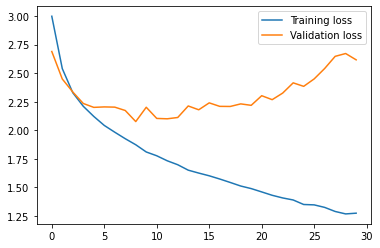
\includegraphics[width=8cm]{images/BasicoLoss.png}
\caption{}
\label{fig:2figsA}}
\begin{minipage}{8cm}
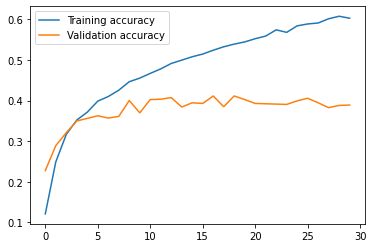
\includegraphics[width=8cm]{images/BasicoAcc.png}
\caption{}
\label{fig:2figsB}
\end{minipage}
\end{figure}
Entrenado durante 30 épocas, vemos que el test tiene una precisión del 38.71$\%$ y la función de périda da 2.589, una predicción mala, aunque este es sólo el modelo base. También podemos observar cómo se produce overfitting, fijándonos en que el accuracy y el loss son mucho mejores en el conjunto train.


\section*{Apartado 2: Mejora del modelo BaseNet}
Para este apartado, mejoramos el modelo propuesto en la guía de prácticas para obtener una mejor accuracy. En las pruebas intermedias de mejoras he usado 30 épocas.

\subsection*{Normalización de datos}
En esta mejora usamos la clase ImageDataGenerator de la que hablamos anteriormente en la explicación de la función \texttt{entrenarModelo}. Para este apartado, queremos que los datos tengan la misma media, 0, y la misma varianza, 1, y simplificar así el entrenamiento. Para ello, creamos una instancia de la clase y establecemos \texttt{featurewise$\_$center y\\ featurewise$\_$std$\_$normalization} a \texttt{True} en la llamada al constructor así como\\ \texttt{validation$\_$split = 0.1} para la validación.
Aplicamos a train la normalización con \texttt{datagen.fit} y al conjunto test con \texttt{datagen.standardize}. Volviendo a ejecutar con esta normalización obtenemos:\\
\begin{center}
Test accuracy: 0.37400001287460327\\
Test loss: 3.0099644660949707
\end{center}
\begin{figure}[H]
\centering
\parbox{8cm}{
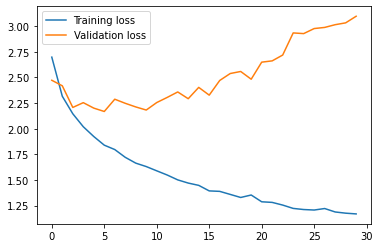
\includegraphics[width=8cm]{images/NormalizacionDeDatosLoss.png}
\caption{}
\label{fig:2figsA}}
\begin{minipage}{8cm}
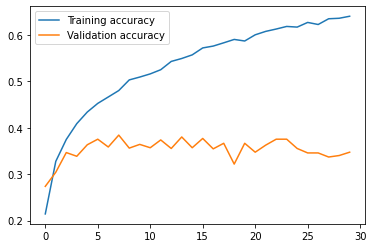
\includegraphics[width=8cm]{images/NormalizacionDeDatosAcc.png}
\caption{}
\label{fig:2figsB}
\end{minipage}
\end{figure}
Una precisión un poco por debajo del modelo base, pero no importa pues facilita y hace más sólido el entrenamiento.

\subsection*{Aumento de datos}
Para evitar que la red se ajuste demasiado al conjunto train, hacemos data augmentation donde cambiamos aleatoriamente algunas fotos de entrenamiento por otras que han sido ligeramente transformadas, por ejemplo rotadas, recortadas o con zoom. Así conseguimos que no memorice tanto las imágenes de entrenamiento sino sus características al tener que varias imágenes ligeramente modificadas responden a la misma etiqueta. Sólo lo hacemos al conjunto de train. Esto se establece también en el constructor de ImageDataGenerator donde cada valor de \texttt{width$\_$shift$\_$range, height$\_$shift$\_$range, zoom$\_$range} indica el rango de la transformación. Por ejemplo, \texttt{height$\_$shift$\_$range = 0.1} indica que mueve la imagen horizontalmente hacia la izquierda o derecha de forma aleatoria en un 10$\%$ del tamaño de la imagen. También permitimos que se pueda hacer un volteo horizontal con \texttt{horizontal$\_$flip} puesto a \texttt{True}. Con estos cambios, obtenemos los siguientes datos:
\\
\begin{center}
Test accuracy: 0.4212000072002411\\
Test loss: 1.985841989517212
\end{center}
\begin{figure}[H]
\centering
\parbox{8cm}{
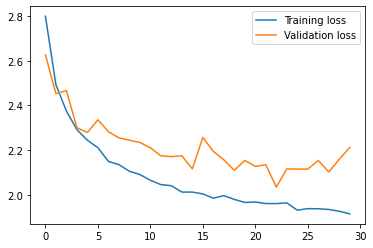
\includegraphics[width=8cm]{images/AumentoDeDatosLoss.png}
\caption{}
\label{fig:2figsA}}
\begin{minipage}{8cm}
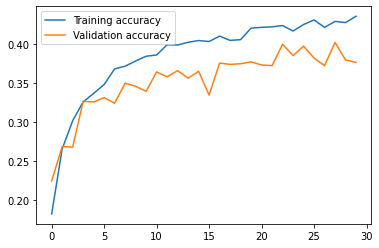
\includegraphics[width=8cm]{images/AumentoDeDatosAcc.png}
\caption{}
\label{fig:2figsB}
\end{minipage}
\end{figure}
Como podemos ver no sólo mejora la precisión del modelo sino que también baja el sobreajuste: las curvas de validación y train están más pegadas y no hay tanta diferencia entre la precisión en el trainning y en el test como la había en el modelo base.


\subsection*{Aumento de profundidad}
Para este apartado, he dividido las convoluciones con un tamaño de kernel (5, 5) en dos de (3, 3) y después de estas he puesto \texttt{MaxPooling2D} para evitar ponerlo después de todas las convoluciones. Además he añadido una convolución final antes de las últimas capas Dense (que las he mantenido igual que en el modelo base). En padding he puesto \texttt{'same'} para no perder la dimensión en las imágenes demasiado rápido. Ahora, tras la ejecución, devuelve los siguientes resultados:
\\
\begin{center}
Test accuracy: 0.631600022315979\\
Test loss: 1.24598228931427
\end{center}
\begin{figure}[H]
\centering
\parbox{8cm}{
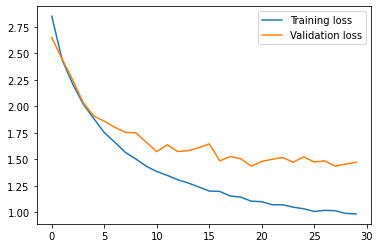
\includegraphics[width=8cm]{images/AumentoProfundidadLoss.png}
\caption{}
\label{fig:2figsA}}
\begin{minipage}{8cm}
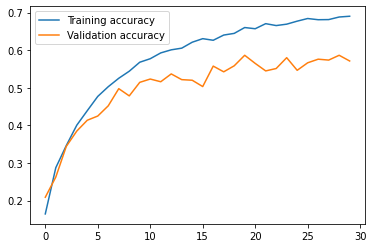
\includegraphics[width=8cm]{images/AumentoProfundidadAcc.png}
\caption{}
\label{fig:2figsB}
\end{minipage}
\end{figure}
Mejora bastante la precisión del modelo y se mantiene con menos overfitting que al principio.

\section*{Batchnormalization}
Estas capas mantienen la media cercana a 0 y la varianza a 1 de las salidas de las capas convolucionales. Como mejor me han funcionado es poniéndolas entre las capas convolucionales y la activación ReLU, aunque tras mirar en varios foros (\href{https://stackoverflow.com/questions/34716454/where-do-i-call-the-batchnormalization-function-in-keras}{ForoDiscusion1}, \href{https://www.reddit.com/r/MachineLearning/comments/67gonq/d_batch_normalization_before_or_after_relu/}{ForoDiscusion2}) he visto que ponerlas antes o despues de la activación es un tema aún abierto. Devuelven los siguientes resultados, donde sube la precisión ligeramente:
\\
\begin{center}
Test accuracy: 0.6895999908447266\\
Test loss: 1.1053860187530518
\end{center}
\begin{figure}[H]
\centering
\parbox{8cm}{
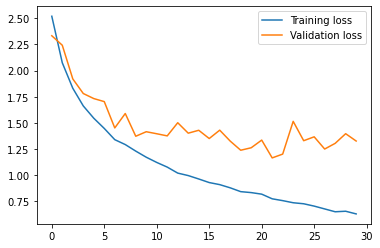
\includegraphics[width=8cm]{images/BatchnormalizationLoss.png}
\caption{}
\label{fig:2figsA}}
\begin{minipage}{8cm}
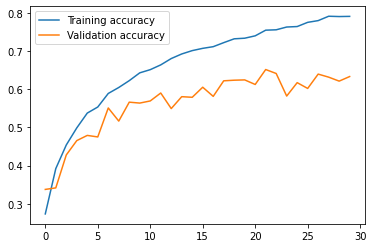
\includegraphics[width=8cm]{images/BatchnormalizationAcc.png}
\caption{}
\label{fig:2figsB}
\end{minipage}
\end{figure}

\subsection*{Dropout}
Añadimos capas de regularización dropout después de las convoluciones para prevenir el overfitting. Es técnica desactiva un a parte de las neuronas temporalmente durante el entrenamiento volviendo a la red menos sensible a los pesos específicos de las neuronas y resultando así en una red capaz de generalizar mejor y con ello, reducir el sobreajuste. El parámetro de esta capa es el porcentaje de neuronas de entrada que se desactivan (0 ninguna y 1 todas). Veamos los resultados que nos devuelve:
\\
\begin{center}
Test accuracy: 0.6948000192642212\\
Test loss: 1.024166226387024
\end{center}
\begin{figure}[H]
\centering
\parbox{8cm}{
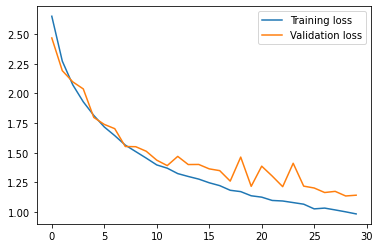
\includegraphics[width=8cm]{images/DropoutLoss.png}
\caption{}
\label{fig:2figsA}}
\begin{minipage}{8cm}
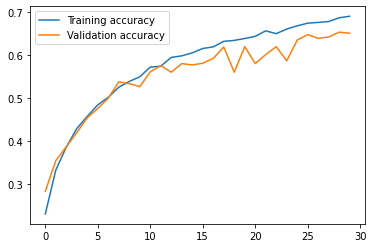
\includegraphics[width=8cm]{images/DropoutAcc.png}
\caption{}
\label{fig:2figsB}
\end{minipage}
\end{figure}
Como vemos, la precisión no cambia mucho pues no es el objetivo de Dropout, pero las curvas de validación y train están mucho más juntas, así como la precisión del conjunto train y test (al rededor de 0.7) lo que indica que se ha reducido el overfitting.

\subsection*{Mejora conjunta}
Ahora como mejora final, y juntándola con el resto de mejoras anteriores del modelo, aplicamos EarlyStopping. Esto nos permite parar el entrenamiento cuando durante un número determinado de épocas (las que indique el parámetro \texttt{patience}, en este caso establecida a 15) no ha mejorado la precisión o el error y recuperamos los mejores pesos hasta el momento con \texttt{restore$\_$best$\_$weights}. Esto sirve para tener menos tiempo de entrenamiento "inútil" cuando el modelo realmente no está aprendiendo ni mejorando la precisión ni el error.\\
Juntando esta última mejora con las anteriores y entrenando durante un máximo de 100 épocas (si no para antes EarlyStopping) conseguimos estos resultados:\\
\begin{center}
Mejores pesos obtenidos en la época 78\\
Test accuracy: 0.753600001335144\\
Test loss: 0.8629369139671326\\
\end{center}
\begin{figure}[H]
\centering
\parbox{8cm}{
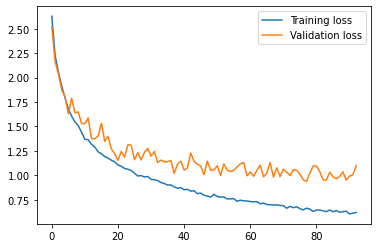
\includegraphics[width=8cm]{images/MejoraConjuntaLoss.png}
\caption{}
\label{fig:2figsA}}
\begin{minipage}{8cm}
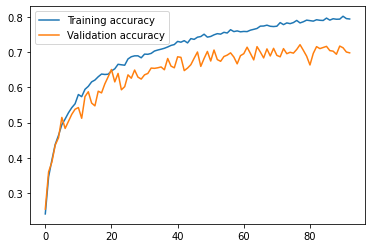
\includegraphics[width=8cm]{images/MejoraConjuntaAcc.png}
\caption{}
\label{fig:2figsB}
\end{minipage}
\end{figure}
Obtenemos una precisión del 75'36$\%$ con lo que prácticamente hemos doblado la del modelo base gracias a estas mejoras. También ha aumentado el tiempo de cómputo, como cabía esperar, de unos 2 segundos a unos 7 en google colab y hemos reducido considerablemente el overfitting.\\
Para acabar este apartado, incluyo una tabla con la arquitectura final del modelo mejorado:\\

\begin{table}[H]
\begin{tabular}{lllcc}
\textbf{Layer No.} & \textbf{Layer Typer} & \textbf{Kernel size} & \textbf{\begin{tabular}[c]{@{}c@{}}Input | Output\\ dimension\end{tabular}} & \textbf{\begin{tabular}[c]{@{}c@{}}Input | Output\\ channels\end{tabular}} \\
1                  & Conv2D               & 3                    & 32|32                                                                       & 3|32                                                                       \\
2                  & BatchNorm            & -                    & 32|32                                                                       & -                                                                          \\
3                  & Relu                 & -                    & 32|32                                                                       & -                                                                          \\
4                  & Conv2D               & 3                    & 32|30                                                                       & 32|32                                                                      \\
5                  & BatchNorm            & -                    & 30|30                                                                       & -                                                                          \\
6                  & Relu                 & -                    & 30|30                                                                       & -                                                                          \\
7                  & MaxPooling2D         & 2                    & 30|15                                                                       & -                                                                          \\
8                  & Dropout              & -                    & 15|15                                                                       & -                                                                          \\
9                  & Conv2D               & 3                    & 15|15                                                                       & 32|64                                                                      \\
10                 & BatchNorm            & -                    & 15|15                                                                       & -                                                                          \\
11                 & Relu                 & -                    & 15|15                                                                       & -                                                                          \\
12                 & Conv2D               & 3                    & 15|13                                                                       & 64|64                                                                      \\
13                 & BatchNorm            & -                    & 13|13                                                                       & -                                                                          \\
14                 & Relu                 & -                    & 13|13                                                                       & -                                                                          \\
15                 & MaxPooling2D         & 2                    & 13|6                                                                        & -                                                                          \\
16                 & Dropout              & -                    & 6|6                                                                         & -                                                                          \\
17                 & Conv2D               & 3                    & 6|6                                                                         & 64|128                                                                     \\
18                 & BatchNorm            & -                    & 6|6                                                                         & -                                                                          \\
19                 & Relu                 & -                    & 6|6                                                                         & -                                                                          \\
20                 & Dropout              & -                    & 6|6                                                                         & -                                                                          \\
21                 & Dense                & -                    & 4608|50                                                                     & -                                                                          \\
22                 & BatchNorm            & -                    & 50|50                                                                       & -                                                                          \\
23                 & Relu                 & -                    & 50|50                                                                       & -                                                                          \\
24                 & Dense                & -                    & 50|25                                                                       & -                                                                         
\end{tabular}
\end{table}
$\rightarrow$Tabla con la arquitectura del modelo mejorado\\
\newpage
\section*{Apartado 3: Transferencia de modelos y ajuste fino con ResNet50 para la base de datos
Caltech-UCSD}
En este último apartado, usamos redes preentrenadas para entrenar con el conjunto de datos Caltech-UCSD, compuesto de 6033 imágenes de 200 especies de pájaros, es decir, 200 clases, con 3000 imágenes en el conjunto de entrenamiento y 3033 en el de prueba. De nuevo, dejamos un 10$\%$ del conjunto trainning para validación.\\
La filosifía que se sigue para usar una red preentrenada es que las primeras capas capturan características más bien generales de la imagen y son las últimas capas las que se adaptan al problema completo. De esta forma, eliminando las últimas capas de la red preentrenada, podemos concatenarla con una red de nuestra elección y adaptarla a nuestro problema, ahorrando tiempo de entrenamiento.\\\\
Como en el anterior apartado, tenemos ya definidas una serie de funciones para leer las imágenes, cargar los datos y mostrar la evolución. Reutilizamos las funciones \texttt{compilar}, \texttt{entrenarModelo} (aunque esta vez sin EarlyStopping ya que el número de épocas a entrenar será bajo) y \texttt{prediccionTest} para evaluar el modelo en el conjunto test.

\subsection*{Resnet50 como extraxtor de características}
Para usar Resnet50 como extractor de características, eliminamos la última capa softmax y utilizamos los datos que nos devuelva como entrada para un nuevo modelo. Esta salida la podemos ver como una colección de características que ya se ha encargado la red preentrenada de obtener.\\
Así, en este apartado hacemos lo siguiente: primero obtenemos el modelo resnet preentrenado en la base de datos ImageNet, le quitamos la última capa y le pasamos nuestros conjuntos train y test para obtener las características de nuestra base de datos (vector de 2048 características) y las usamos como entrada de un modelo simple que compilamos, entrenamos y evaluamos.\\\\
Consigo esto mediante la función \texttt{resnet$\_$extractor$\_$car} que entrena, evalúa y muestra resultados de nuestro modelo pasándole las características extraídas. Tiene dos opciones: usar un modelo simple o uno más sofisticado para hacer el primer subapartado A. Para el B, usamos una función igual que la anterior descrita, \texttt{resnet$\_$extractor$\_$carB} pero usando otro modelo.
\subsubsection*{Apartado 1}
A.-\\
Empezamos este subapartado con un modelo más simple para luego compararlo con otro algo más complejo. El modelo simple consta de una capa final fully-connected de tamaño 200 y activación softmax. Ejecutando durante 15 épocas esta capa obtenemos estos resultados:\\\\
\begin{center}
Test accuracy: 0.41707879304885864\\
Test loss: 2.5126025676727295
\end{center}
\begin{figure}[H]
\centering
\parbox{8cm}{
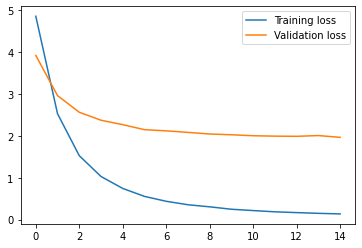
\includegraphics[width=8cm]{images/Resnet1A2Loss.png}
\caption{}
\label{fig:2figsA}}
\begin{minipage}{8cm}
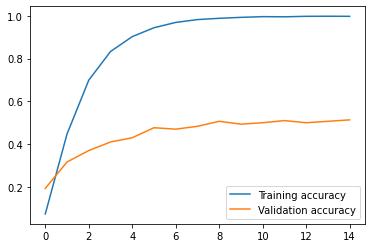
\includegraphics[width=8cm]{images/Resnet1A2Acc.png}
\caption{}
\label{fig:2figsB}
\end{minipage}
\end{figure}
Vemos que hay mucho sobreajuste así que entrenar durante más épocas no tendría sentido pues no mejoraría los resultados.\\
Ahora probamos un modelo algo más complejo con una capa más totalmente conectada. El modelo sigue esta arquitectura:\\
\begin{table}[H]
\begin{tabular}{lllcc}
\textbf{Layer No.} & \textbf{Layer Typer} & \textbf{Kernel size} & \textbf{\begin{tabular}[c]{@{}c@{}}Input | Output\\ dimension\end{tabular}} & \textbf{\begin{tabular}[c]{@{}c@{}}Input | Output\\ channels\end{tabular}} \\
1                  & Dense                & -                    & 2048||1024                                                                  & -                                                                          \\
2                  & Relu                 & -                    & 1024|1024                                                                   & -                                                                          \\
3                  & Dense                & -                    & 1024|512                                                                    & -                                                                          \\
4                  & Relu                 & -                    & 512|512                                                                     & -                                                                          \\
5                  & Dropout              & -                    & 512|512                                                                     & -                                                                          \\
6                  & Dense                & -                    & 512|200                                                                     & -                                                                         
\end{tabular}
\end{table}
Sigue siendo un modelo simple pero con algo más de profundidad y vemos que mejora ligeramente el modelo más simple:\\
\begin{center}
Test accuracy: 0.43125617504119873\\
Test loss: 2.3488149642944336\\
\end{center}
\begin{figure}[H]
\centering
\parbox{8cm}{
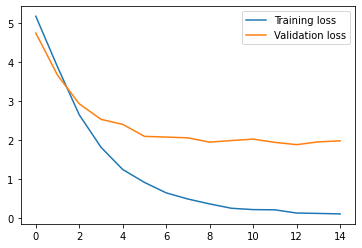
\includegraphics[width=8cm]{images/Resnet1A1Loss.png}
\caption{}
\label{fig:2figsA}}
\begin{minipage}{8cm}
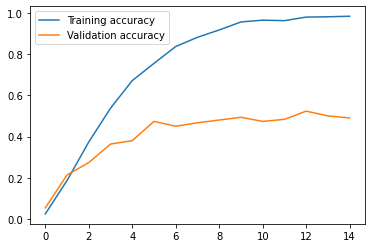
\includegraphics[width=8cm]{images/Resnet1A1Acc.png}
\caption{}
\label{fig:2figsB}
\end{minipage}
\end{figure}
B.-\\
El último modelo que probamos es algo más complejo:\\
\texttt{def modeloB():
  model = Sequential()
  model.add(Conv2D(1024,\\
                     kernel$\_$size = (3, 3),
                     input$\_$shape = (7,7,2048,)))\\
  model.add(BatchNormalization())\\
  model.add(Activation('relu'))\\
  model.add(MaxPooling2D(pool$\_$size=(2, 2)))\\
  model.add(Flatten())\\
  model.add(Dropout(0.25))\\
  model.add(Dense(512, activation='relu'))\\
  model.add(BatchNormalization())\\
  model.add(Dropout(0.25))\\
  model.add(Dense(218, activation='relu'))\\
  model.add(BatchNormalization())\\
  model.add(Dropout(0.5))\\
  model.add(Dense(200, activation='softmax'))\\
  return model}
\\\\Como vemos, hay una primera capa convolucional y \texttt{BatchNormalization} antes de cada capa de activación Relu, así como \texttt{Dropout} y las capas filanes fully-connected. También al crear el modelo ResNet50 hace falta pasarle el parámetro \texttt{pooling=None} para que se elimine el AveragePooling como se pide en el enunciado de la práctica. Con todo ello, obetenemos los siguientes resultados:\\
\begin{center}
Test accuracy: 0.41707879304885864\\
Test loss: 2.3695855140686035\\
\end{center}
\begin{figure}[H]
\centering
\parbox{8cm}{
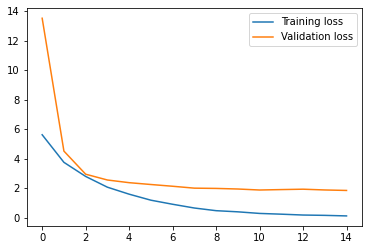
\includegraphics[width=8cm]{images/Resnet1BLoss.png}
\caption{}
\label{fig:2figsA}}
\begin{minipage}{8cm}
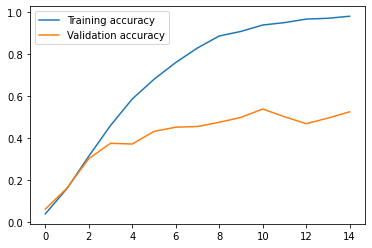
\includegraphics[width=8cm]{images/Resnet1BAcc.png}
\caption{}
\label{fig:2figsB}
\end{minipage}
\end{figure}
No conseguimos mejorar el accuracy y se sigue produciendo overfitting. Además cada época tarda varios segundos en vez de los milisegundos que tardaba en el apartado A, así que es preferible usar el apartado A.

\subsubsection*{Apartado 2}
En este último apartado se nos pide hacer un ajuste fino de la red ResNet50, así que en vez de extraer las características y pasárselas a un modelo, esta vez consideramos todo el conjunto como un modelo que entrenaremos unas cuantas épocas, es decir, al entrenar adaptaremos los pesos de la red preentrenada (que ya de por sí son buenos) a la nuestra. El modelo que usamos aquí es uno sencillo con una capa FC, un Dropout y un softmax final. Sería la función siguiente:\\
\texttt{def modeloFT(modelo):\\
    modelo = Dense(1024, activation = 'relu') (modelo)\\ 
    modelo = Dropout(0.5) (modelo)\\
    modelo = Dense(200, activation = 'softmax') (modelo)\\
    return modelo}
Para crear ese modelo, instanciamos un modelo mediante \texttt{Model} con entrada la ResNet50 y como salida, la de nuestro modelo anterior. Todo ello, lo he hecho en una función llamada \texttt{resnetFT} donde ejecuta el apartado por completo: crea los datagen y el modelo, lo entrena durante 12 épocas y lo evalúa mostrando los resultados sobre el test e historial de entrenamiento.
\begin{center}
Test accuracy: 0.45070886611938477\\
Test loss: 2.3895986080169678\\
\end{center}
\begin{figure}[H]
\centering
\parbox{8cm}{
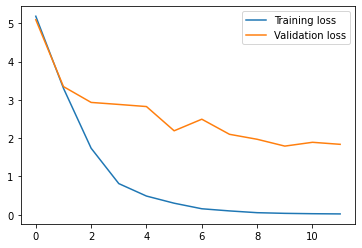
\includegraphics[width=8cm]{images/Resnet2Loss.png}
\caption{}
\label{fig:2figsA}}
\begin{minipage}{8cm}
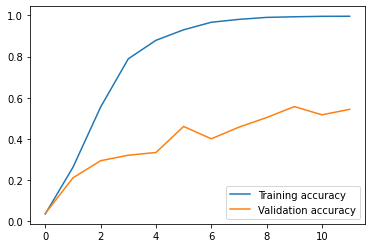
\includegraphics[width=8cm]{images/Resnet2Acc.png}
\caption{}
\label{fig:2figsB}
\end{minipage}
\end{figure}
El resultado es similar al del apartado anterior: se genera overfitting muy rápido y no conseguimos mejorar mucho el accuracy con respecto a anteriores resultados. La conclusión es que al estar la red ya preentrenada, no hay mucho entrenamiento "extra" que podamos hacer así que los modelos nos darán todos resultados parecidos.\\

\section*{Bonus}
Para el bonus me he centrado en reducir el overfitting de los datos sin que ello afecte mucho al accuracy. Esto lo he conseguido aumentando la profundidad del modelo: he añadido en total cuatro bloques convolucion-convolucion-batchnormalization-relu-dropout, tres de ellos con un Maxpooling, y al final tres bloques Dense. En vez de Flatten he utilizado GlobalAveragePooling2D que me devuelve mejores resultados en el accuracy. También para reducir aún más el overfitting he añadido al data augmentation el cizallamiento en el datagen y la posibilidad de rotar imágenes. El modelo se puede ver en \texttt{modeloBonus} y la ejecución del bonus en la función \texttt{bonus}. Con todo ello, he conseguido eliminar el overfitting y obtener unos resultados de accuracy y los casi tan buenos como en el apartado 2.\\
\begin{center}
Test accuracy: 0.6952000260353088\\
Test loss: 1.0124149322509766
\end{center}
\begin{figure}[H]
\centering
\parbox{8cm}{
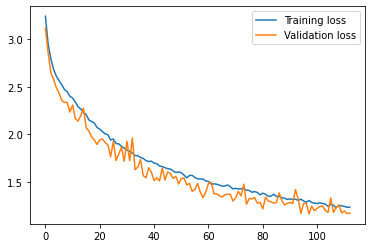
\includegraphics[width=8cm]{images/BonusLoss.png}
\caption{}
\label{fig:2figsA}}
\begin{minipage}{8cm}
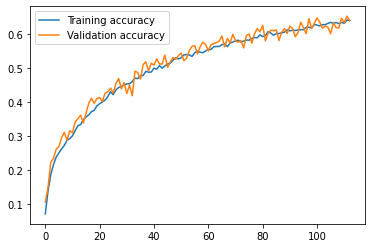
\includegraphics[width=8cm]{images/BonusAcc.png}
\caption{}
\label{fig:2figsB}
\end{minipage}
\end{figure}
Vemos cómo la curva de validación siempre permanece junto a la de trainnig indicando que el overfitting ha desaparecido.
% --------------------------------------------------------------
%     You don't have to mess with anything below this line.
% --------------------------------------------------------------
 
\end{document}